\documentclass{standalone}
\usepackage{pgfplots}
\usepgfplotslibrary{groupplots}
% Required packages and libraries
\usepackage{tikz}
\usetikzlibrary{decorations.pathreplacing,calligraphy}
	
\usepackage{pgfplotstable}	
	
	\usepackage{color}
	\usepackage{tikz}
	\usepackage{graphicx}
	\usepackage{amsmath}
	
	\usetikzlibrary{shapes,decorations,arrows,calc,arrows.meta,fit,positioning}

\begin{document}
	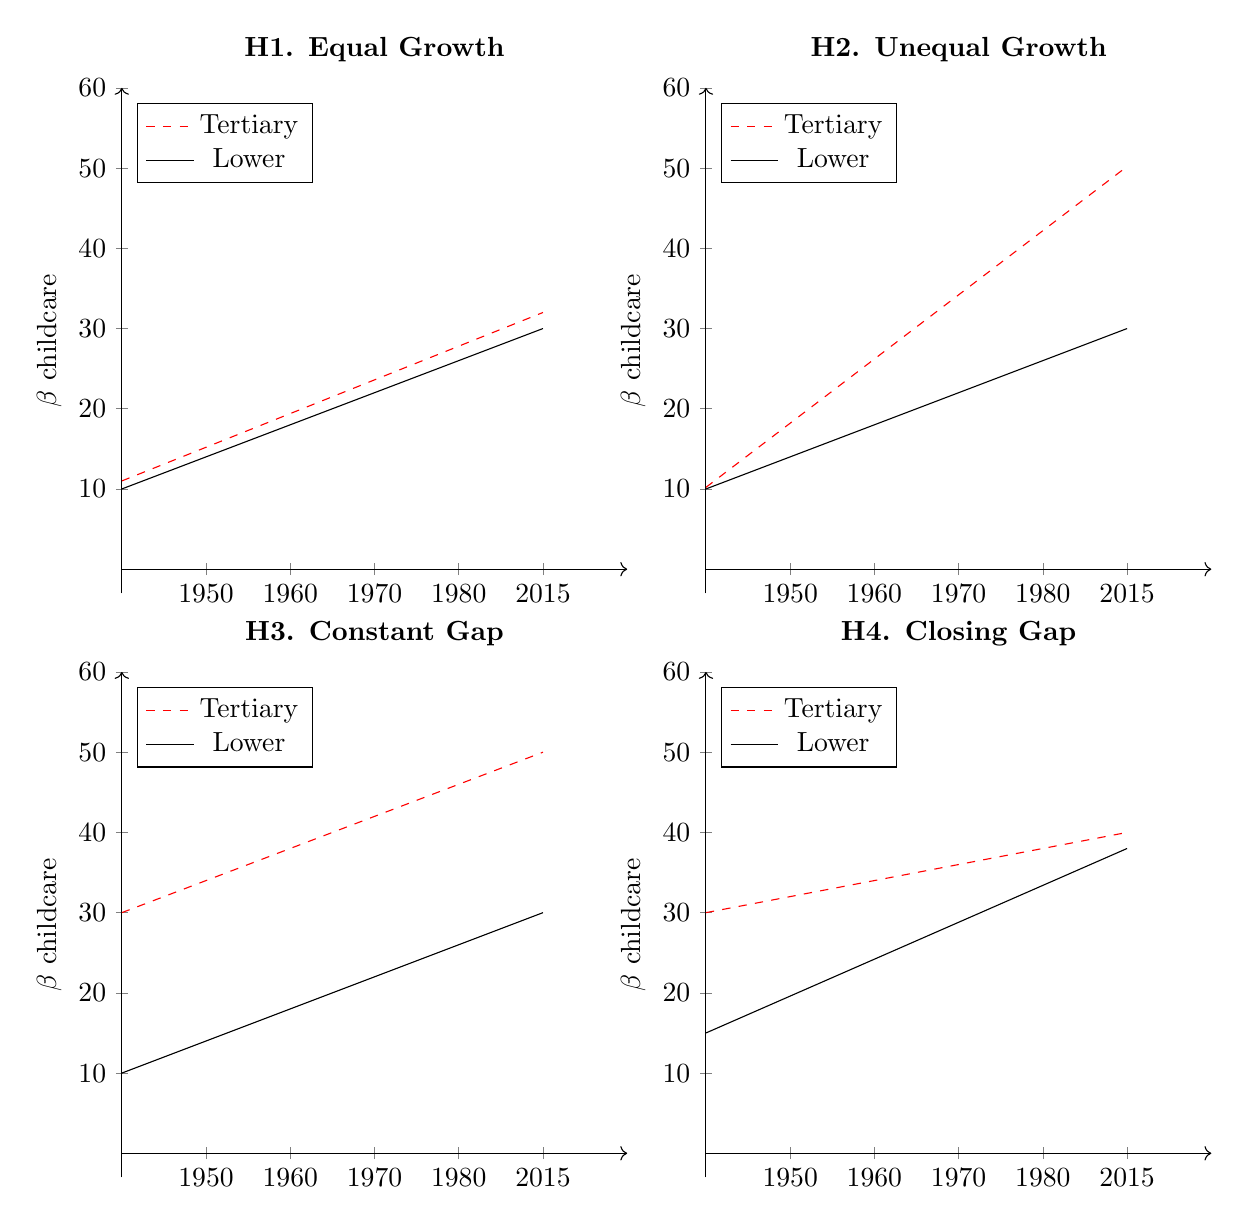
\begin{tikzpicture}
	\begin{groupplot}[
	group style={group size=2 by 2},
	height=8cm,
	width=8cm,
		xmin=0,
		xmax=12,
		xtick={2, 4, 6, 8, 10},
		xticklabels={$1950$, $1960$, $1970$, $1980$, $2015$},
		ymin=-3,ymax=60,
		legend entries={Tertiary, Lower},
		legend pos=north west,
		axis lines=middle,
		axis line style={->},
		x label style={at={(axis description cs:0.5,-0.1)},anchor=north},
		y label style={at={(axis description cs:-0.1,.5)},rotate=90,anchor=south},
		xlabel={},
		ylabel={$\beta$ childcare}]
		axis lines = left]
		group size=2 by 2,
		xlabels at=edge bottom,
		ylabels at=edge left]
	\nextgroupplot[title=\textbf{H1. Equal Growth}]
		\addplot [ domain=0:10, style = dashed, samples=30, color=red]{11 + x*2.1};
			\addplot [ domain=0:10, style = solid, samples=30, color=black]{10 + x*2};
	\nextgroupplot[title=\textbf{H2. Unequal Growth}]
		\addplot [ domain=0:10, style = dashed, samples=30, color=red]{10.2 + x*4};
	\addplot [ domain=0:10, style = solid, samples=30, color=black]{10 + x*2};
	\nextgroupplot[title=\textbf{H3. Constant Gap}]
	\addplot [ domain=0:10, style = dashed, samples=30, color=red]{30 + x*2};
	\addplot [ domain=0:10, style = solid, samples=30, color=black]{10 + x*2};
	\nextgroupplot[title=\textbf{H4. Closing Gap}]
	\addplot [ domain=0:10, style = dashed, samples=30, color=red]{30 + x*1};
	\addplot [ domain=0:10, style = solid, samples=30, color=black]{15 + x*2.3};
	\end{groupplot}
	\end{tikzpicture}
\end{document}